\documentclass[12pt]{article}
\usepackage[a4paper, margin=.30in]{geometry}
\usepackage{graphicx ,
            wrapfig,
            xcolor, 
            enumerate,
            amsmath,fontenc,makecell,chemfig, multirow
            }

\newcommand\headerMe[2]{\noindent{}#1\hfill#2}
\renewcommand{\thesection}{\Roman{section}}

%\title{Leçon N 6 : Le mouvement}
\author{Zakaria HAOUZAN}
\date{\today}

\begin{document}
% headers --------------
\headerMe{Matière : Physique-Chimie}{Professeur : Zakaria HAOUZAN}\\
\headerMe{Unité : Travail Mécanique et Energie }{Établissement : Lycée SKHOR qualifiant}\\
\headerMe{Niveau : TCS}{Heure : 2H}\\

% ------Content ________
\begin{center}

    \Large{Leçon $N^{\circ} 6 $: \color{red} Classification périodique des éléments chimiques }
\end{center}

%\begin{wrapfigure}[10]{r}{0.5\textwidth}
%    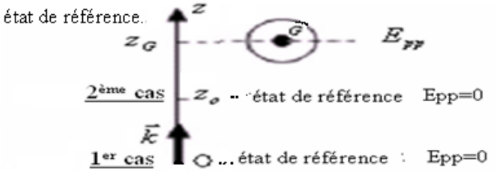
\includegraphics[width=0.5\textwidth]{./img/img00.png}
%\end{wrapfigure}

\section{Situation problème :  }
Dès le début du 19ème siècle, les éléments
chimiques deviennent de plus en plus
nombreux, ce qui a poussé les scientifiques à
essayer de les classer, et de les regrouper.

Comment les éléments chimiques sont-
ils regroupés ?

Quelle est l’utilité de la classification
périodique des éléments chimiques ?

\section{Classification périodique des éléments chimiques }
\subsection{Classification périodique selon
MENDELEÏEV }

Dans l'année 1860, un jeune chimiste russe Dimitri
Ivanovitch MENDELEÏEV, propose une première
classification périodique des éléments chimiques qui
contenait 63 éléments qui étaient connus à l’époque,
en les rangeant par deux critères principaux :
\\ - Classer les éléments chimiques par ordre de
masses atomiques croissantes
\\ - Les éléments chimiques figurant dans une même
colonne présentent des propriétés chimiques
similaires

Mendeleïev prévoyait l’existence d’éléments
chimiques inconnus à l’époque, où il plaçait à ses
places un point d’interrogation ( ? ). Ils ont été
découverts plus tard et leurs propriétés étaient
identiques à celles déjà prévu par Mendeleïev. Comme
le Germanium, découvert en 1886

\subsection{Classification périodique actuelle : }
Le tableau périodique actuel comporte des lignes horizontales appelées périodes dont le
nombre est 7, et des colonnes verticales appelées groupes dont le nombre est 18. Le tableau
périodique actuel est basé sur les critères suivants :

\begin{itemize}
    \item Les éléments chimiques sont classés par l’ordre du numéro atomique Z croissant
    \item Chaque période comporte les atomes qui ont le même nombre de couches
électroniques occupées. Le nombre de couches électroniques occupées représente le 
numéro de la période. 1ère période: couche K, 2ème période: couche L, 3ème période: couche M.
\item Chaque groupe comporte les atomes qui ont le même nombre d’électrons sur leurs
couches externes. Le nombre d’électrons sur les couches externes représente le numéro
du groupe. Les atomes des éléments du groupe (I) ont 1 électron sur la couche externe,
ceux du groupe (II) ont 2 électrons sur la couche externe, etc...
\end{itemize}

\begin{center}
    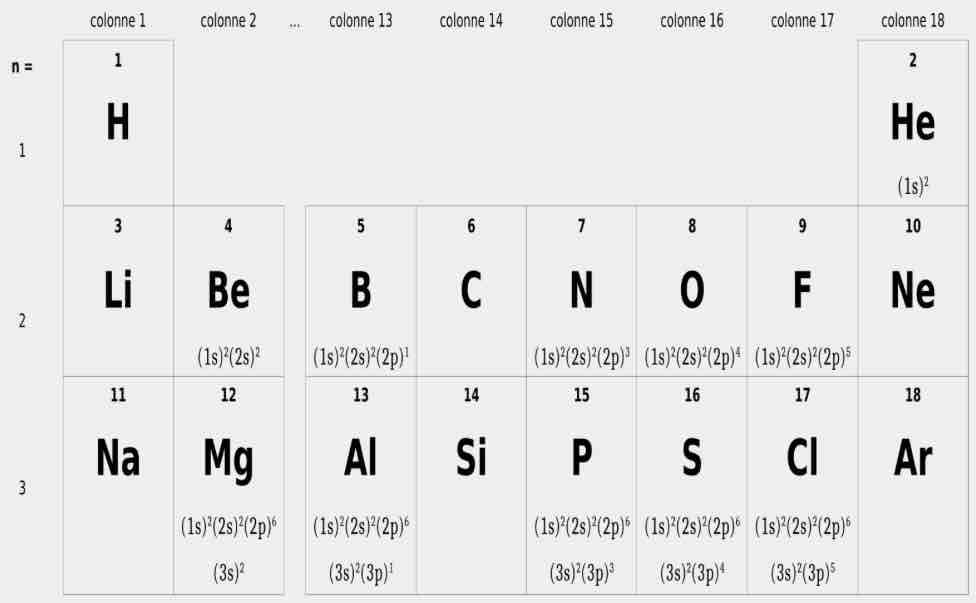
\includegraphics[width=0.5\textwidth]{./img/img00.jpg}
\end{center}

\section{Utilisation du tableau périodique des éléments chimiques : }
\subsection{Les familles chimiques : }
Une famille chimique est constituée de l’ensemble des éléments chimiques
appartenant à un même groupe du tableau périodique. Ces éléments
possèdent des propriétés chimiques similaires
 \begin{enumerate}
     \item[a .]\textbf{Famille des métaux Alcalins :} C’est le groupe (I), à l’exception de l’hydrogène H, il contient Li, Na, K ... Ces éléments
possèdent 1 électron sur leurs couches électroniques externes. Ils donnent des ions $Li^+,Na^+,K^+$ ... Ce sont des métaux mous
\item[b .] \textbf{Famille des métaux Alcalino-terreux } : C’est le groupe (II), il contient Be, Mg, Ca ... Ces éléments possèdent 2 électrons sur leurs
couches électroniques externes. Ils donnent des ions $Be^{2+}, Mg^{2+}, Ca^{2+}...$
\item[c .] \textbf{Famille des Halogènes : } C’est le groupe (VII), il contient F, Cl, Br, I ... Ces éléments possèdent 7 électrons sur leurs
couches électroniques externes. Ils donnent des ions $F^-, Cl^-, Br^-, I^- $... Ils existent dans la nature sous la forme de molécules diatomiques $F_2, Cl_2, Br_2, I_2$.
\item[d .] \textbf{Famille des gaz rares : }C’est le groupe (VIII), il contient He, Ne, Ar ... Ces éléments possèdent une grande stabilité
chimique c-à-d ils ne réagissent pas car leurs couches externes sont saturées
 \end{enumerate}
\subsection{Autres utilisations :  }La classification périodique des éléments chimiques permet de 
\begin{itemize}
    \item Prédire les réactions chimiques possibles dans lesquelles les éléments chimiques
appartenant au même groupe peuvent-être participés
\\Exemple :

$4Li + O_2 \rightarrow 2Li_2O$ \hspace{1cm} $4Na + O_2 \rightarrow 2 Na_2O $ \hspace{1cm} $4K + O_2 \rightarrow 2K_2O$
\item Déterminer la formule chimique des ions monoatomiques qui sont susceptible de se
former à partir des éléments chimiques appartenant au même groupe
\item Déterminer la formule chimique des molécules dans lesquelles les éléments chimiques
appartenant au même groupe peuvent-être donnés
\\Exemple : 
L’atome de carbone C se combine avec 4 atomes d’hydrogène H pour donner une
molécule $CH_4$
L’atome de silicium Si se combine avec 4 atomes d’hydrogène H pour donner une
molécule $SiH_4$

\end{itemize}

\section{Exercice d’application :}

La couche électronique externe d'un atome est la couche (L). Elle comporte 7 électrons.
\begin{enumerate}
    \item Dans quelle période et quel groupe de la classification périodique appartient l'élément chimique correspondant ?
    \item Donner son numéro atomique et l'identifier.
    \item Quel ion monoatomique est susceptible de se former à partir de cet atome? Justifier.
    \item Nommer la famille à laquelle cet élément chimique appartient. Citer deux éléments
appartenant à la même famille

\end{enumerate}





\end{document}

